\section{Petersson 内积}
\label{sec:petersson}
% ============================================================================

\textbf{出发点。}
前几节已经建立了 Hecke 算子 $T_n$ 作用于 $\Sk_k$ 的代数结构。
接下来自然的问题是：$\Sk_k$ 是否有一个自然的\emph{内积}，使得 $T_n$ 对此内积是自伴的？
有了自伴性，就能用有限维内积空间的谱定理：$T_n$ 可对角化，
从而 $\Sk_k$ 有正交的特征形式基。

\begin{definition}[Petersson 内积]
\label{def:petersson}
设 $\mathcal{F}$ 是 $\SL_2(\Z)$ 的标准基本域，$\Gamma = \SL_2(\Z)$，$f, g \in \Sk_k(\Gamma)$。
定义
\[
  \langle f, g \rangle
  = \int_{\mathcal{F}} f(\tau)\overline{g(\tau)}\, (\mathrm{Im}\,\tau)^k
    \frac{dx\,dy}{y^2},
  \quad \tau = x + iy.
\]
其中 $d\mu(\tau) = y^{-2}\,dx\,dy$ 是双曲平面 $\HH$ 上的 $\SL_2(\R)$-不变测度（Poincaré 测度）。
\end{definition}

% TikZ figure: Petersson inner product — fundamental domain integration
% Shows the hyperbolic measure y^{k-2} dx dy on fundamental domain
\begin{figure}[ht]
\centering
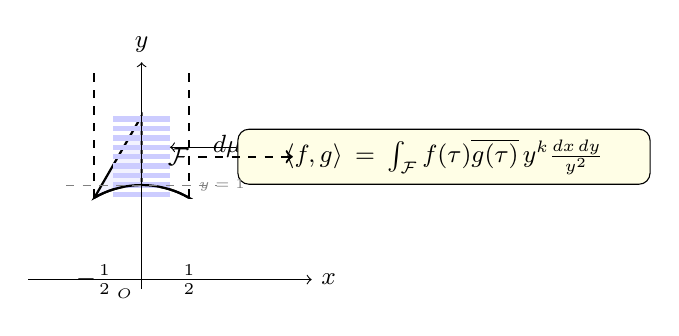
\begin{tikzpicture}[scale=1.2]
  % Draw fundamental domain
  \draw[thick, fill=blue!5] 
    (-0.5, 0.866) arc (120:60:1) -- (0.5, 0.866)
    arc (60:90:1) -- (0, 1.732)
    -- cycle;

  % Shade to indicate integration
  \foreach \y in {0.9, 1.0, 1.1, 1.2, 1.3, 1.4, 1.5, 1.6, 1.7} {
    \draw[blue!20, line width=2pt] (-0.3, \y) -- (0.3, \y);
  }

  % Boundary arcs
  \draw[thick] (-0.5, 0.866) arc (120:60:1);
  \draw[thick, dashed] (-0.5, 0.866) -- (-0.5, 2.2);
  \draw[thick, dashed] (0.5, 0.866) -- (0.5, 2.2);

  % Labels
  \node at (0, 1.3) [right=6pt, font=\small] {$\mathcal{F}$};
  \node at (-0.5, 0) [font=\small] {$-\frac{1}{2}$};
  \node at (0.5, 0) [font=\small] {$\frac{1}{2}$};

  % Hyperbolic measure annotation
  \draw[->] (1.0, 1.4) -- node[right, font=\small] {$d\mu = \frac{dx\,dy}{y^2}$} (0.3, 1.4);

  % Formula below
  \node[draw, rounded corners, fill=yellow!10, font=\small, text width=5cm, align=center]
    at (3.2, 1.3) {$\langle f, g \rangle = \int_{\mathcal{F}} f(\tau)\overline{g(\tau)}\, y^{k} \frac{dx\,dy}{y^2}$};

  % Arrow connecting region to formula
  \draw[->, dashed, thick] (0.6, 1.3) -- (1.6, 1.3);

  % Axes
  \draw[->] (-1.2, 0) -- (1.8, 0) node[right, font=\small] {$x$};
  \draw[->] (0, -0.1) -- (0, 2.3) node[above, font=\small] {$y$};
  \node at (0, 0) [below left, font=\tiny] {$O$};

  % y=1 label
  \draw[gray, dashed] (-0.8, 1) -- (0.8, 1);
  \node at (0.85, 1) [font=\tiny, gray] {$y=1$};
\end{tikzpicture}
\caption{Petersson 内积通过在基本域 $\mathcal{F}$ 上积分定义，
使用双曲测度 $y^{k-2}\,dx\,dy$（即 $y^k \cdot y^{-2}\,dx\,dy$）。}
\label{fig:petersson-domain}
\end{figure}


\textbf{为什么要乘 $y^k$？}
对 $f \in \Sk_k(\Gamma)$，变换律 $f(\gamma\tau) = (c\tau+d)^k f(\tau)$ 成立。
函数 $F(\tau) = |f(\tau)|^2 y^k$ 满足 $F(\gamma\tau) = F(\tau)$，
故 $F$ 是 $\Gamma$-不变函数，从而 $F \cdot d\mu$ 可以在 $\mathcal{F}$ 上良定义积分。
尖点形式在尖点处 $f(\tau) = O(e^{-2\pi y})$，
保证了当 $y \to \infty$ 时被积函数指数衰减，积分收敛。

\begin{proposition}[内积的性质]
\label{prop:petersson-properties}
\begin{enumerate}[(i)]
  \item $\langle \cdot, \cdot \rangle$ 是 $\Sk_k(\Gamma)$ 上的 Hermite 内积（正定）。
  \item 若 $f = \sum a_n q^n$，$g = \sum b_n q^n$，则（粗略近似）
        \[
          \langle f, g \rangle
          \approx \sum_{n=1}^\infty \frac{a_n \overline{b_n}}{n^{k-1}}.
        \]
        （精确的"Rankin-Selberg"方法将内积化成 $L$-函数的值。）
\end{enumerate}
\end{proposition}

\begin{proof}[(i) 的验证]
共轭线性、Hermite 性（$\langle g, f \rangle = \overline{\langle f, g \rangle}$）是显然的。
正定性：$\langle f, f \rangle = \int_\mathcal{F} |f(\tau)|^2 y^k d\mu > 0$ 当 $f \neq 0$，
因为 $|f|^2 y^k > 0$ 除有限个零点外处处正，而被积区域面积为正。
\end{proof}

\begin{theorem}[Hecke 算子的自伴性]
\label{thm:hecke-selfadjoint}
对任意 $n \geq 1$ 和 $f, g \in \Sk_k(\SL_2(\Z))$，
\[
  \langle T_n f, g \rangle = \langle f, T_n g \rangle.
\]
即 $T_n$ 关于 Petersson 内积是自伴算子。
\end{theorem}

\begin{proof}[证明（素数情形 $n = p$）]
利用 $T_p$ 的双陪集分解（\cref{def:hecke-coset}）：
\[
  (T_p f)(\tau) = p^{k-1} \left[
    p^{-k} f(p\tau) + \sum_{b=0}^{p-1} p^{-k} f\!\left(\frac{\tau+b}{p}\right)
  \right].
\]
计算内积需要把对 $\mathcal{F}$ 的积分换成对各陪集代表的积分，
再用 Poincaré 测度的 $\SL_2(\R)$-不变性，
以及 $T_p$ 与"转置"算子（对应 $\begin{pmatrix}p&0\\0&1\end{pmatrix}^T = \begin{pmatrix}1&0\\0&p\end{pmatrix}$）
实际上给出同一个算子（在 $\SL_2(\Z)$ 级别上），这等价于矩阵的对合
$\begin{pmatrix}a&b\\c&d\end{pmatrix}^* = \begin{pmatrix}d&-b\\-c&a\end{pmatrix}$，
可验证 $T_p^* = T_p$。

完整细节见 Diamond \& Shurman §5.4。
\end{proof}

\begin{corollary}[特征形式正交基]
\label{cor:eigenform-basis}
$\Sk_k(\SL_2(\Z))$ 有一组关于 Petersson 内积正交的归一化特征形式基
$\{f_1, \ldots, f_d\}$（$d = \dim \Sk_k$），
即 $T_n f_i = a_n(f_i) f_i$ 对所有 $n$，且 $\langle f_i, f_j \rangle = \delta_{ij}$。
\end{corollary}

\begin{proof}
$\Sk_k$ 是有限维内积空间，$\{T_n\}$ 是一族彼此交换的自伴算子，
由线性代数（交换自伴族可同时对角化）得到正交特征基。
\end{proof}

\begin{example}[$\Sk_{12}$ 的情况]
$\dim \Sk_{12}(\SL_2(\Z)) = 1$，基为 $\Delta$，故 $\Delta$ 自动是特征形式。
没有"正交化"的问题——$\Sk_{12}$ 里只有一条"方向"。

对 $\dim = 2$ 的情形（例如 $\Sk_{16}$，有基 $\{\Delta E_4, \Delta E_{12}\}$），
Hecke 算子 $T_2$ 在此基下有矩阵表示，特征向量给出两个正交特征形式。
\end{example}

\begin{remark}
Petersson 内积不只是代数工具——它与 $L$-函数深度相连。
Rankin-Selberg 方法利用内积计算
$\langle f, f \rangle = c \cdot L(k, f \otimes \bar{f})$（某常数 $c$），
从而把几何（积分）与解析（$L$-函数）完美对接。
\end{remark}
